Die zukünftige Entwicklung von CSP lässt sich in zwei Phasen beschreiben. Zuerst muss eine kommerzieller Anreiz und eine Wettbewerbsfähigkeit auf dem Energiemarkt geschaffen werden. Sollte dies geschehen sein, werden in der zweiten Phase Investoren bereit sein in neue Anlagen zu investieren, was zu einer erhöhten Kapazität und somit zu einer Senkung der Kosten führt. Die zweite Phase ist unter normalen Umständen als Folge einer erfolgreichen Etablierung der Technologie aus Phase Eins anszusehen. Somit liegt der Schlüssel für eine positive Entwicklung in Phase Eins. Um einen kommerziellen Anreiz und Wettbewerb für CSP zu erlangen, ist eine aktive Förderung der Technologien bis zu einem kritischen Punkt nötig. Um diesen Punkt zu erreichen sind vor allem die Bereiche als wichtig anzusehen, die die ökonomischen Eigenschaften eines CSP Projektes betrachten.
Für eine mögliche Entwicklung in der Zukunft wurden von NEEDS (New Energy Externalities Developments for Sustainability) drei verschiedene Szenarien unter Berücksichtigung von verschiedenen Konditionen aufgestellt. Es wird hierbei zwischen einer "`optimistic-realisitc"' Variante und zwei extremen Varianten "`very optimistic"' und "`pessimistic"' unterschieden. Die Szenarien orientieren sich an dem oben vorgestellten Zwei-Phasen Ansatz.

\begin{figure}[H]
	\centering
	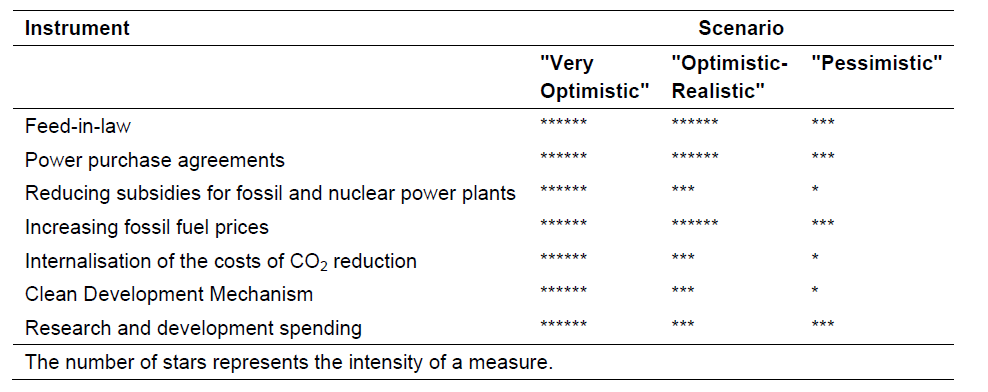
\includegraphics[width=0.9\textwidth,trim=1 1 1 1,clip]{instruments_scenario.png}
	\caption{Szenarien-Parameter~(\cite{viebahn2008})}
	\label{fig:inst}
\end{figure}

Für die Szenarien wird eine Liste von Parametern aufgestellt, die für jedes Szenario unterschiedliche Gewichte erhalten (Abb.~\ref{fig:inst}).

Das "`very optimistic"' Szenario nimmt an, dass in beide Phasen das volle Potential erreicht wird. In der ersten Phase wird also ein früher Anstieg von CSP Kapazitäten erwartet. Hierzu ist ein globales Klimaschutzabkommen notwendig, welches alle erneuerbaren Energien enthält und ein Regelwerk vorsieht.
Zum Vergleich sieht das "`optimistic-realistic"' Szenario kein unmittelbares Erreichen aller möglichen Potentiale in Phase Eins vor. Es geht davon aus, dass sich diese jedoch im Laufe der Zeit aktivieren. Desweiteren wird nicht davon ausgegangen, dass nukleare und fossile Energien völlig verdrängt werden. Durch Einspeisegesetze, unterstützt durch erhöhten Preise für nukleare und fossile Energien, wird jedoch ein Anstieg von CSP prognostiziert.
Der Ansatz für das "`pessimistic"' Szenario sieht eine Verzögerung der Entwicklung von CSP um weitere Dekaden vor. In Phase Eins wird der kritische Punkt nicht erreicht und es wird zu keiner fördernden Entwicklungsphase, noch zu einer resultierenden Phase Zwei kommen. CSP Anlagen werden nicht völlig aus den erneuerbaren Energien verschwinden, jedoch wird nur ein geringer Anstieg bis 2050 vorhergesehen.


\begin{figure}[H]
	\centering
	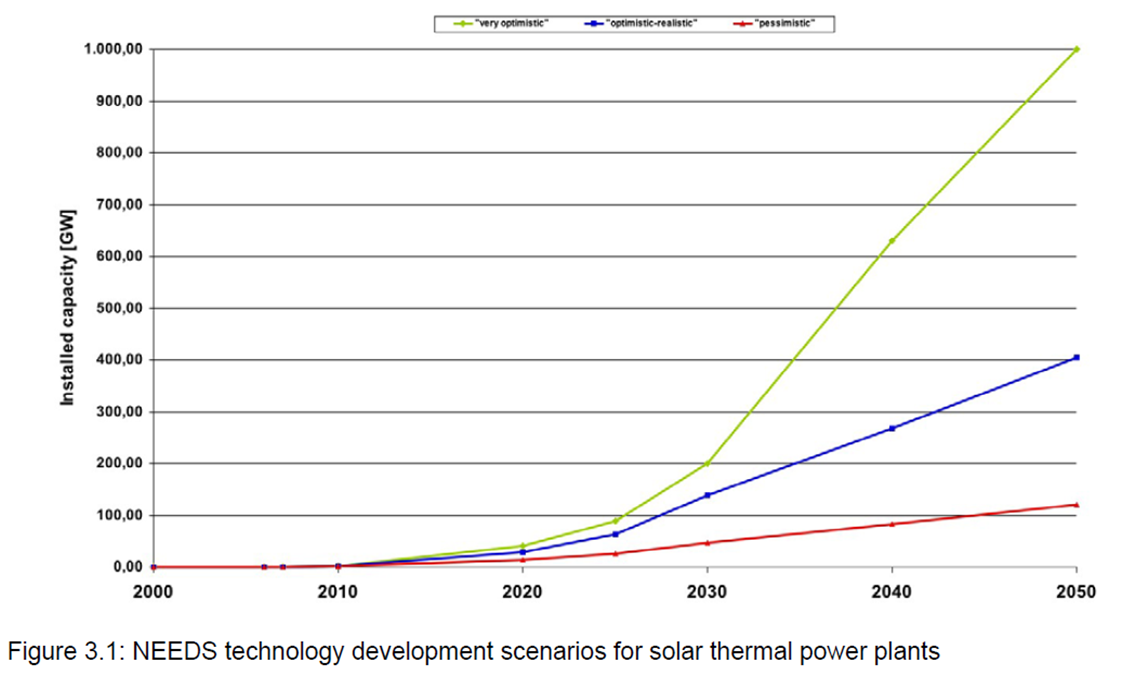
\includegraphics[width=0.9\textwidth,trim=1 1 1 1,clip]{szenarien.png}
	\caption{Ergebnisse der Szenarien-Studie}
	\label{fig:scenes}
\end{figure}


